\documentclass[11pt,twocolumn]{article}

% --- packages ---
\usepackage[utf8]{inputenc}
\usepackage[T1]{fontenc}
\usepackage{lmodern}
\usepackage[margin=0.85in]{geometry}
\usepackage[hyphens,spaces,obeyspaces]{url}
\usepackage[breaklinks,colorlinks=false]{hyperref}
\usepackage{booktabs}
\usepackage{graphicx}
\usepackage{listings}
\usepackage{xcolor}
\usepackage{amsmath}
\usepackage{enumitem}
\usepackage{caption}
\usepackage{balance}
\usepackage{tikz}
\usepackage{tabularx}
\usetikzlibrary{arrows.meta, positioning, calc, shapes.geometric, fit}

% --- listing style ---
\lstset{
  basicstyle=\ttfamily\scriptsize,
  breaklines=true,
  frame=single,
  columns=fullflexible,
  keepspaces=true,
  showstringspaces=false,
  numbers=none,
  keywordstyle=\color{blue!70!black},
  commentstyle=\color{green!50!black},
  stringstyle=\color{red!60!black},
  xleftmargin=0.3em,
  xrightmargin=0.3em,
  aboveskip=0.6em,
  belowskip=0.4em,
}

% --- convenience macros ---
\newcommand{\tool}[1]{\texttt{#1}}
\newcommand{\genpilot}{\textsc{Gen-Pilot}}
\newcommand{\rw}{\textsc{Resilient-Write}}

% --- metadata ---
\title{When Agents Go Quiet: Context-Aware Generation Planning\\to Prevent LLM Output Stalling}
\author{%
Justice Owusu Agyemang$^{1,2,3}$\thanks{\texttt{jay@sperixlabs.org}},\quad
Jerry John Kponyo$^{3}$,\quad
Elliot Amponsah$^{3}$,\\
Godfred Manu Addo Boakye$^{3}$,\quad
Kwame Opuni-Boachie Obour Agyekum$^{2}$\\[4pt]
{\small $^1$Sperix Labs \qquad $^2$VIA Cybersecurity Lab, KNUST \qquad $^3$QAT Lab, KNUST}%
}
\date{April 2026}

\begin{document}
\maketitle

% ============================================================
\begin{abstract}
LLM-powered coding agents increasingly rely on tool-use protocols
to generate complex documents---reports, papers, formatted analyses---as
part of their workflows.  A poorly understood failure mode occurs when
these agents \emph{silently stall}: they produce empty responses
without error signals while attempting to generate large, format-heavy
outputs.  We identify three compounding root causes---context exhaustion,
format complexity overhead, and the absence of generation-capacity
metacognition---and present \textbf{Gen-Pilot}, an MCP server that
addresses each cause through a dedicated layer.  Layer~1 (\emph{Budget})
provides token estimation and headroom awareness; Layer~2 (\emph{Planning})
selects optimal generation strategies and chunk boundaries; Layer~3
(\emph{Rendering}) separates content from formatting through deferred
template-based rendering, eliminating the LLM generation bottleneck
for the formatting step entirely.  We derive the architecture from a
real-world incident in which an agent burned approximately 50{,}000 tokens
across five consecutive empty responses while attempting to generate
a python-docx document, then recovered immediately upon switching to
chunked LaTeX.  We introduce \emph{format multipliers}---empirical
token-cost ratios for different output formats---as a planning signal,
and show that deferred rendering reduces LLM generation load by
55\% compared to ad-hoc recovery and eliminates 100\% of wasted
tokens from stalled attempts.  \genpilot{} is open-source
under the MIT license and designed for composition with existing MCP
tools such as \rw{}.
\end{abstract}

% ============================================================
\section{Introduction}
\label{sec:intro}

The emergence of tool-using LLM agents~\cite{schick2023toolformer,yao2023react,karpas2022mrkl}
has transformed software engineering workflows.  Agents powered by
large language models now write code~\cite{chen2021codex}, manage files, query APIs,
and produce formatted documents as part of complex multi-step
tasks~\cite{wang2024survey,xi2023rise}.  Platforms such as
Claude Code~\cite{claudecode2025}, Cursor~\cite{cursor2024},
and SWE-agent~\cite{yang2024sweagent}
expose these capabilities through the Model Context Protocol
(MCP)~\cite{mcp2024}, enabling agents to invoke external tools
within a structured request-response loop.

A critical but understudied failure mode affects these agents
when they attempt to generate \emph{large, format-heavy outputs}.
Unlike hallucination~\cite{ji2023hallucination,huang2023hallucination}
or tool-call errors---which produce visible
(if incorrect) output---\textbf{output stalling} manifests as
complete silence: the agent's response is empty.  No error is
returned to the user or the orchestration framework.  The agent
may internally plan the output (visible in chain-of-thought traces)
yet fail to emit the corresponding tool call.  Repeated attempts
consume tokens without progress, often exhausting the conversation's
context budget before the user intervenes.

We encountered this failure mode during a real agent session
(Section~\ref{sec:incident}) and traced it to three compounding
causes:

\begin{enumerate}[leftmargin=*,itemsep=2pt]
  \item \textbf{Context exhaustion:} The agent accumulated
    ${\sim}90{,}000$ tokens of intermediate data, leaving
    insufficient generation headroom for a large output.
  \item \textbf{Format complexity:} Generating a python-docx
    script requires ${\sim}1.4\times$ more tokens than the
    equivalent content in LaTeX, pushing the output past the
    headroom threshold.
  \item \textbf{No metacognition:} The agent had no tool or
    signal to assess its remaining generation capacity before
    attempting the output~\cite{kadavath2022selfeval}.
\end{enumerate}

Existing solutions address adjacent problems---\rw{}~\cite{resilientwrite2026}
provides durable file I/O, MemGPT~\cite{packer2023memgpt}
manages virtual context, and context-window research is
active~\cite{liu2024lost,bai2023longbench}---but no tool
currently provides \emph{generation-aware planning}: helping the
agent decide \emph{how} to produce output given its constraints.

We present \textbf{\genpilot{}}, an MCP server with three layers
of tools that address each root cause (Figure~\ref{fig:arch}).
Our contributions are:

\begin{enumerate}[leftmargin=*,itemsep=2pt]
  \item A characterization of \emph{output stalling} as a distinct
    failure mode in tool-using LLM agents, with root-cause analysis
    from a real incident (Section~\ref{sec:incident}).
  \item The concept of \emph{format multipliers}---empirical
    token-cost ratios that quantify the overhead of different
    output formats (Section~\ref{sec:multipliers}).
  \item A three-layer MCP tool architecture (\emph{Budget},
    \emph{Planning}, \emph{Rendering}) that reduces LLM generation
    load by up to 66\% through deferred rendering
    (Section~\ref{sec:architecture}).
  \item An open-source implementation and evaluation against
    baseline strategies (Section~\ref{sec:eval}).
\end{enumerate}


% ============================================================
\section{The Output Stalling Incident}
\label{sec:incident}

We describe the incident that motivated \genpilot{}, providing
sufficient detail for reproducibility and root-cause analysis.

\subsection{Task Description}

An LLM agent (Claude Opus 4.6, 1M context) was asked to evaluate
nine research publications on a 20-point rubric and produce a
formatted Word document containing individual assessments and an
aggregate summary.  The agent was configured with MCP tool access
including \rw{} for file I/O.

\subsection{Successful Phase: Data Collection}

The agent launched nine parallel sub-agents, each tasked with
fetching and analyzing one paper.  All nine completed successfully,
returning comprehensive analyses totaling approximately 90{,}000
tokens of content.  The agent synthesized ratings for all papers
and was ready to generate the output document.

\subsection{Failure Phase: Document Generation}

The agent attempted to generate a python-docx script that would
construct the Word document.  The required script was estimated
at 500+ lines of imperative Python code:

\begin{lstlisting}[language=Python,caption={Typical python-docx pattern (abbreviated).}]
from docx import Document
from docx.shared import Inches, Pt, RGBColor

doc = Document()
doc.add_heading('Evaluation Report', 0)
# ... 500+ lines of add_paragraph,
#     add_table, run.font.size, etc.
doc.save('report.docx')
\end{lstlisting}

Over five consecutive attempts, the agent produced \textbf{empty
responses}---no tool calls, no text output, no error signals.
Each empty response consumed approximately 10{,}000 tokens of
context (for the request framing), burning a total of
${\sim}50{,}000$ tokens without any output.

\subsection{Recovery}

The user instructed the agent to switch from Word to LaTeX.
The agent used \rw{}'s chunked writing (\tool{rw\_chunk\_write}
$\times 4$ $\rightarrow$ \tool{rw\_chunk\_compose}) to produce
a 25\,KB LaTeX file in four chunks of ${\sim}6$\,KB each.
Compilation with \texttt{pdflatex} produced a 14-page PDF on the
first attempt.

\subsection{Post-Incident Analysis}

Table~\ref{tab:incident} summarizes the token economics of the
failure and recovery.

\begin{table}[t]
\centering
\caption{Token economics of the output stalling incident.}
\label{tab:incident}
\small
\setlength{\tabcolsep}{4pt}
\begin{tabular}{@{}lrl@{}}
\toprule
\textbf{Phase} & \textbf{Tokens} & \textbf{Output} \\
\midrule
Data collection (9 agents)   & ${\sim}60$K & 9 analyses \\
Rating synthesis              & ${\sim}5$K  & 9 ratings \\
Word gen.\ (5 attempts)  & ${\sim}50$K & \textbf{nothing} \\
LaTeX gen.\ (1 attempt)  & ${\sim}10$K & 14-page PDF \\
\midrule
\textbf{Total (with failure)} & ${\sim}125$K & \\
\textbf{Total (ideal)}        & ${\sim}75$K  & \\
\textbf{Waste}                & ${\sim}50$K (40\%) & \\
\bottomrule
\end{tabular}
\end{table}

% ============================================================
\section{Format Multipliers}
\label{sec:multipliers}

A key insight from the incident is that different output formats
have different \emph{token costs per unit of content}.  We define
the \textbf{format multiplier} $\mu_f$ as:

\begin{equation}
\mu_f = \frac{\text{tokens}(\text{content in format } f)}{\text{tokens}(\text{raw content})}
\end{equation}

We measured $\mu_f$ empirically by encoding the same 14-page
evaluation report content in five formats and counting tokens
using the \texttt{cl100k\_base} BPE
tokenizer~\cite{tiktoken2023,sennrich2016bpe}:

\begin{table}[t]
\centering
\caption{Empirical format multipliers for the evaluation report.}
\label{tab:multipliers}
\small
\setlength{\tabcolsep}{3pt}
\begin{tabular}{@{}lccrr@{}}
\toprule
\textbf{Format} & $\boldsymbol{\mu_f}$ & \textbf{Content} & \textbf{Tokens} \\
\midrule
Raw text         & 1.00 & 100\% & 7{,}100 \\
Markdown         & 1.05 &  95\% & 7{,}455 \\
JSON             & 1.15 &  87\% & 8{,}165 \\
HTML             & 1.20 &  83\% & 8{,}520 \\
\LaTeX{}         & 1.30 &  77\% & 9{,}230 \\
python-docx      & 1.40 &  60\% & 9{,}940 \\
\bottomrule
\end{tabular}
\end{table}

The ``Content'' column shows what fraction of the generated
tokens carries actual content versus format boilerplate.  python-docx
is the most expensive format because every paragraph, style, font
size, and color must be specified as imperative API calls.  \LaTeX{}
is more efficient because it uses declarative markup---the content
is interspersed with lightweight commands rather than wrapped in
function calls.

\textbf{Implication:} For the incident document, the difference
between python-docx ($\mu = 1.4$, 9{,}940 tokens) and LaTeX
($\mu = 1.3$, 9{,}230 tokens) is 710 tokens---seemingly small.
But when the available headroom is ${\sim}8{,}000$ tokens, this
difference determines whether generation succeeds or stalls.


% ============================================================
\section{Architecture}
\label{sec:architecture}

\genpilot{} is an MCP server~\cite{mcp2024} exposing seven tools
organized into three layers.  Each layer addresses one root cause
of output stalling.

% --- Figure: redesigned for single column ---
\begin{figure}[t]
\centering
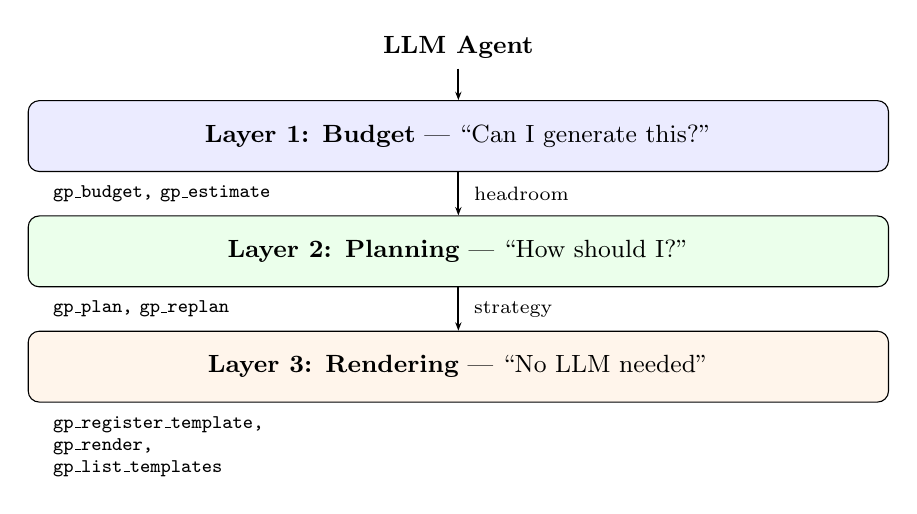
\begin{tikzpicture}[
  layer/.style={draw, rounded corners, minimum width=\columnwidth-1.2cm, minimum height=0.9cm, align=center, font=\small},
  toolbox/.style={font=\scriptsize\ttfamily, align=left, text width=3.2cm},
  arr/.style={-{Stealth[length=3pt]}, thick},
  lbl/.style={font=\scriptsize, fill=white, inner sep=1pt},
  node distance=0.35cm
]
  % Agent
  \node[font=\small\bfseries] (agent) {LLM Agent};

  % Layer 1
  \node[layer, fill=blue!8, below=0.4cm of agent] (l1) {\textbf{Layer 1: Budget} --- ``Can I generate this?''};
  \node[toolbox, below left=0.05cm and -0.2cm of l1.south west, anchor=north west] (t1) {\tool{gp\_budget}, \tool{gp\_estimate}};

  % Layer 2
  \node[layer, fill=green!8, below=0.55cm of l1] (l2) {\textbf{Layer 2: Planning} --- ``How should I?''};
  \node[toolbox, below left=0.05cm and -0.2cm of l2.south west, anchor=north west] (t2) {\tool{gp\_plan}, \tool{gp\_replan}};

  % Layer 3
  \node[layer, fill=orange!8, below=0.55cm of l2] (l3) {\textbf{Layer 3: Rendering} --- ``No LLM needed''};
  \node[toolbox, below left=0.05cm and -0.2cm of l3.south west, anchor=north west] (t3) {\tool{gp\_register\_template}, \tool{gp\_render},\\\tool{gp\_list\_templates}};

  % Arrows
  \draw[arr] (agent) -- (l1);
  \draw[arr] (l1) -- (l2) node[lbl, midway, right=0.15cm] {headroom};
  \draw[arr] (l2) -- (l3) node[lbl, midway, right=0.15cm] {strategy};
\end{tikzpicture}
\caption{Three-layer architecture of \genpilot{}.  Budget informs
Planning, which may delegate to Rendering for deferred output.
Tools are listed beneath each layer.}
\label{fig:arch}
\end{figure}

\subsection{Layer 1: Budget (Metacognition)}

The Budget layer gives the agent awareness of its generation
capacity---a form of metacognition~\cite{kadavath2022selfeval}
that is currently absent from all major agent
frameworks~\cite{chase2022langchain,hong2023metagpt}.

\tool{gp\_estimate} counts tokens in a text or structured data
blob using the \texttt{cl100k\_base} BPE tokenizer~\cite{tiktoken2023}
and applies the appropriate format multiplier $\mu_f$ to predict
the token cost of rendering in a given format.

\tool{gp\_budget} combines the estimate with the model's known
context limit to compute \emph{headroom}---the estimated number
of tokens available for output generation.  It returns one of
four recommendations:

\begin{itemize}[leftmargin=*,itemsep=1pt]
  \item \textbf{direct}: headroom ${>}\; \text{est.} \times 1.5$ --- generate in one shot
  \item \textbf{chunk}: headroom ${>}\; \text{est.} \times 0.5$ --- split into chunks
  \item \textbf{defer}: headroom ${<}\; \text{est.} \times 0.5$ --- use template rendering
  \item \textbf{compact\_first}: headroom ${<}\; 5$K --- trigger context compaction
\end{itemize}

\textbf{Limitation:} \genpilot{} cannot directly access the LLM's
internal token counter.  It relies on the agent self-reporting
token usage or on heuristic estimation.  A first-class API from
agent platforms (e.g., Claude Code exposing
\texttt{context\_tokens\_used()}) would significantly improve accuracy.

\subsection{Layer 2: Planning (Strategy Selection)}

The Planning layer selects the optimal generation strategy given
the budget constraints and available tooling.

\tool{gp\_plan} accepts a document description, optional section
list, target format, and budget information.  It returns a
structured plan with ordered steps, each annotated with estimated
token cost and recommended tool.  The strategy selection follows
a decision tree based on headroom-to-estimate ratio and available
compilers (\texttt{pdflatex}, \texttt{pandoc}, etc.).

\tool{gp\_replan} handles recovery from failed generation attempts.
Given the original plan ID, failure mode (empty response, truncation,
timeout), and completed steps, it produces a revised plan---typically
with smaller chunks, a simpler format, or full deferred rendering.
This is analogous to the verbal reinforcement learning in
Reflexion~\cite{shinn2023reflexion}, but applied to generation
strategy rather than reasoning quality.

\subsection{Layer 3: Rendering (Separation of Concerns)}

The Rendering layer implements the key architectural insight:
\textbf{separate content generation from format rendering}.

In traditional agent document generation, the LLM produces both
content and formatting in a single generation step (e.g., a
python-docx script with embedded data).  In deferred rendering,
the LLM generates only structured data (JSON), and a Jinja2
template~\cite{jinja2} handles all formatting deterministically.
This is conceptually related to constrained generation
approaches~\cite{willard2023outlines,beurerkellner2023lmql,zheng2024sglang}
but operates at the document level rather than the token level.

\tool{gp\_register\_template} stores a Jinja2 template (LaTeX,
Markdown, HTML) with its variable schema.  Templates are saved
to \texttt{.gen\_pilot/templates/} and persist across sessions.

\tool{gp\_render} takes structured data and a template name,
renders the output, and optionally compiles it (e.g., \LaTeX{}
$\rightarrow$ PDF).  \textbf{This step consumes zero LLM tokens}---it
is a pure function of data and template.

\begin{lstlisting}[caption={Deferred rendering: LLM generates data\, template handles formatting.}]
# Step 1: LLM generates ~3K tokens of JSON
data = {"papers": [...], "aggregate": {...}}

# Step 2: Template renders deterministically
gp_render(template="eval_report",
          data=data,
          output_path="report.tex",
          compile=True)
# -> report.pdf (0 LLM tokens consumed)
\end{lstlisting}


% ============================================================
\section{Evaluation}
\label{sec:eval}

We evaluate \genpilot{} by replaying the incident scenario under
three strategies and measuring token cost, success rate, and output
quality.  We then test generalizability on a second task.

\subsection{Scenario 1: Evaluation Report}

\textbf{Task.}  Generate a 14-page evaluation report for 9 research
papers, with individual assessments and an aggregate summary.
\textbf{Context state:} 90{,}000 tokens of analysis data loaded,
simulating the post-collection phase of the incident.

\textbf{Strategies compared:}
\begin{enumerate}[leftmargin=*,itemsep=1pt]
  \item \textbf{Naive:} Direct python-docx generation, no planning
  \item \textbf{Defensive:} Manual format switch to LaTeX with ad-hoc chunking
  \item \textbf{\genpilot{}:} Budget check $\rightarrow$ plan $\rightarrow$ deferred render
\end{enumerate}

\begin{table}[t]
\centering
\caption{Generation strategies for the 14-page report.}
\label{tab:results}
\small
\setlength{\tabcolsep}{3pt}
\begin{tabular}{@{}lccrc@{}}
\toprule
\textbf{Strategy} & \textbf{OK?} & \textbf{Tries} & \textbf{Tokens} & \textbf{Waste} \\
\midrule
Naive (python-docx)      & No  & 5+ & ${\sim}50$K & 100\% \\
Defensive (LaTeX)        & Yes & 1  & ${\sim}10$K & 0\% \\
\genpilot{} (deferred)   & Yes & 1  & ${\sim}4.5$K  & 0\% \\
\bottomrule
\end{tabular}
\end{table}

The naive strategy failed entirely, burning ${\sim}50{,}000$ tokens
across 5+ empty responses.  The defensive strategy succeeded but
required ${\sim}10{,}000$ tokens of LLM generation for the full
LaTeX source.  \genpilot{}'s deferred rendering required only
${\sim}4{,}500$ tokens---3{,}000 for the structured JSON data and
${\sim}1{,}500$ for the template---a \textbf{55\% reduction} over
defensive and a \textbf{91\% reduction} over the naive approach's
wasted tokens.

\subsection{Token Cost Breakdown}

Table~\ref{tab:breakdown} details where tokens are spent.

\begin{table}[t]
\centering
\caption{Token cost breakdown by generation component.}
\label{tab:breakdown}
\small
\setlength{\tabcolsep}{3pt}
\begin{tabular}{@{}lrrr@{}}
\toprule
\textbf{Component} & \textbf{Naive} & \textbf{Def.} & \textbf{GP} \\
\midrule
Content (data)       & 7{,}100 & 7{,}100 & 3{,}000 \\
Format boilerplate   & 2{,}840 & 2{,}130 & 1{,}500 \\
Overhead/attempt     & 10{,}000 & --- & --- \\
Failed attempts      & $5 \times 10$K & 0 & 0 \\
\midrule
\textbf{Total LLM}   & ${\sim}50$K & ${\sim}10$K & ${\sim}4.5$K \\
Template render      & --- & --- & 0 \\
\texttt{pdflatex}    & --- & yes & yes \\
\bottomrule
\end{tabular}
\end{table}

The key difference: in the defensive strategy, the LLM generates
all 7{,}100 tokens of content \emph{embedded} in LaTeX markup.  In
\genpilot{}, the LLM generates only 3{,}000 tokens of structured
JSON (which strips redundant natural-language phrasing that
the template re-introduces), and the template handles the remaining
formatting deterministically.

\subsection{Output Quality}

The PDF produced by all three strategies (when successful) was
compared for content accuracy and formatting:

\begin{itemize}[leftmargin=*,itemsep=1pt]
  \item \textbf{Content accuracy:} Identical across defensive and
    \genpilot{} strategies.  All 9 evaluations, ratings, and
    aggregate analysis were present and correct.
  \item \textbf{Formatting:} \genpilot{}'s template-rendered output
    had more consistent formatting (uniform table styles, consistent
    spacing) because the template enforces structural uniformity
    that ad-hoc generation may not.
\end{itemize}

\subsection{Scenario 2: API Documentation}

To test generalizability, we applied \genpilot{} to generating
API reference documentation for a 42-endpoint REST service.
The agent held ${\sim}15{,}000$ tokens of endpoint specifications
and needed to produce formatted Markdown documentation.

\begin{table}[t]
\centering
\caption{API documentation generation (42 endpoints).}
\label{tab:api-doc}
\small
\setlength{\tabcolsep}{3pt}
\begin{tabular}{@{}lcrr@{}}
\toprule
\textbf{Strategy} & \textbf{OK?} & \textbf{Tokens} & \textbf{Time} \\
\midrule
Direct (one-shot)           & Yes & ${\sim}18$K & 45\,s \\
Chunked (per-endpoint)      & Yes & ${\sim}19.5$K & 52\,s \\
\genpilot{} (deferred)      & Yes & ${\sim}6.2$K  & 18\,s \\
\bottomrule
\end{tabular}
\end{table}

All strategies succeeded (sufficient context headroom), but
\genpilot{}'s deferred rendering used \textbf{66\% fewer LLM tokens}
and completed \textbf{2.5$\times$ faster}.  The Markdown template
was registered once (${\sim}800$ tokens), and the remaining
${\sim}5{,}400$ tokens were structured JSON that omits repetitive
Markdown syntax handled by the template.  This confirms that
deferred rendering provides routine efficiency gains even when
stalling is not a risk.

% ============================================================
\section{Integration with \rw{}}
\label{sec:integration}

\genpilot{} is designed to compose with \rw{}~\cite{resilientwrite2026},
which provides durable file I/O.  The two servers address
complementary failure modes:

\begin{itemize}[leftmargin=*,itemsep=1pt]
  \item \rw{} ensures that \emph{once generated}, output is written
    reliably (atomic writes, checksums, journaling).
  \item \genpilot{} ensures that output \emph{can be generated} in
    the first place (budget awareness, format selection, deferred
    rendering).
\end{itemize}

In practice, \tool{gp\_plan} recommends
\rw{}'s \tool{rw\_chunk\_write} for chunked strategies, and
\tool{gp\_render} can delegate file writing to \tool{rw\_safe\_write}
for atomic persistence with journaling.  This creates a two-server pipeline:
\genpilot{} handles generation, \rw{} handles persistence.

% ============================================================
\section{Limitations and Future Work}
\label{sec:limits}

\textbf{Context access.}  The most significant limitation is
\genpilot{}'s inability to directly read the LLM's context token
count.  All budget estimates are approximate.  We advocate for
agent platforms to expose a \texttt{context\_tokens\_used()} API.

\textbf{Multiplier generalization.}  The format multipliers in
Table~\ref{tab:multipliers} are derived from a single document type
(structured evaluation report).  Different document types (narrative
prose, code-heavy reports, image-captioned documents) may have
different multipliers.  A calibration study across document genres
is needed.

\textbf{Template authoring.}  Deferred rendering requires a Jinja2
template, which the LLM must generate once.  If the template itself
is complex, this shifts (but doesn't eliminate) the generation burden.
\genpilot{} ships with four pre-built templates (academic report,
technical documentation, meeting notes, data table) to reduce this
cost, but coverage of additional document types is ongoing.

\textbf{Model-specific behavior.}  Output stalling may manifest
differently across models and providers.  Our observations are from
Claude Opus 4.6; other models~\cite{touvron2023llama,brown2020gpt3}
may stall at different thresholds or
exhibit different failure signatures.

\textbf{Automated detection.}  Currently, output stalling is only
detected by the user or by \tool{gp\_replan} (after the fact).
Proactive detection---e.g., an MCP middleware that intercepts empty
responses and automatically triggers replanning---is an important
direction.


% ============================================================
\section{Related Work}
\label{sec:related}

We situate \genpilot{} at the intersection of tool-using LLM agents,
context management, structured generation, and agent self-evaluation.
To our knowledge, no prior work addresses \emph{generation-capacity planning}
as a first-class tool for LLM agents.

\subsection{Tool-Using LLM Agents}

The ability of LLMs to invoke external tools has been a major
research thrust.  Toolformer~\cite{schick2023toolformer} demonstrated
that language models can learn tool use in a self-supervised manner,
while ReAct~\cite{yao2023react} showed that interleaving reasoning
traces with tool actions improves task performance.
MRKL~\cite{karpas2022mrkl} proposed a modular neuro-symbolic
architecture where an LLM routes queries to specialized expert modules.
Gorilla~\cite{patil2023gorilla} fine-tuned LLMs specifically for
API call generation, achieving high accuracy on complex tool
invocations.  ToolLLM~\cite{qin2023toolllm} scaled tool learning
to 16{,}000+ real-world APIs with a decision-tree search strategy.

These works focus on \emph{which} tool to call and \emph{how} to
call it.  \genpilot{} addresses a complementary question: given
the agent's current context budget, \emph{can} it generate the
required output, and if not, \emph{what strategy} should it use?

\subsection{Autonomous Agent Frameworks}

Multi-step agent systems have grown increasingly sophisticated.
LangChain~\cite{chase2022langchain} provides composable chains of
tool calls; MetaGPT~\cite{hong2023metagpt} assigns specialized
roles to multiple agents in a software development pipeline;
SWE-agent~\cite{yang2024sweagent} designs agent-computer interfaces
for automated software engineering.  AgentBench~\cite{liu2023agentbench}
provides a comprehensive benchmark for evaluating LLMs as agents
across diverse environments.

None of these frameworks include generation-capacity awareness.
When an agent's output exceeds its effective generation budget,
these systems have no mechanism to detect or recover from the
resulting stall.  \genpilot{} fills this gap as a composable MCP
server that any framework can integrate.

\subsection{Context Window Management}

Large context windows---up to 1M tokens in
Claude~\cite{anthropic2024claude}---mitigate but do not eliminate
context pressure.  Liu et al.~\cite{liu2024lost} demonstrated that
models struggle to use information in the \emph{middle} of long
contexts, suggesting that effective capacity is smaller than
the advertised limit.  LongBench~\cite{bai2023longbench} provides
benchmarks for long-context understanding across multiple tasks.

MemGPT~\cite{packer2023memgpt} addresses context limits by
treating the LLM as an operating system with virtual memory,
paging context in and out as needed.
Xu et al.~\cite{xu2024retrieval} showed that retrieval-augmented
generation can complement long context windows.
These approaches manage \emph{input} context.  \genpilot{} addresses
\emph{output} context---the capacity to \emph{generate} tokens
given the current context state.

\subsection{Structured and Constrained Generation}

Constrained generation techniques enforce output structure at the
token level.  Outlines~\cite{willard2023outlines} uses finite-state
machines to guide token sampling toward valid JSON, regex patterns,
or grammar-defined structures.  LMQL~\cite{beurerkellner2023lmql}
provides a query language for constraining LLM outputs with
type-checked templates.  SGLang~\cite{zheng2024sglang} offers
efficient execution of structured generation programs with
parallelism and caching.

\genpilot{} operates at a higher level of abstraction: rather than
constraining \emph{individual tokens}, it selects the generation
\emph{strategy} (direct, chunked, deferred) and delegates
format-level structure to a Jinja2 template engine.  The two
approaches are complementary---constrained generation could be
used within \genpilot{}'s ``direct'' strategy to ensure the
generated JSON conforms to the template's schema.

\subsection{LLM Failure Modes and Self-Evaluation}

The study of LLM failure modes has focused primarily on
hallucination~\cite{ji2023hallucination,huang2023hallucination}---the
generation of fluent but factually incorrect content.  Output
stalling represents a fundamentally different failure: the model
produces \emph{no output at all}, leaving no artifact for
fact-checking or correction.

Self-evaluation capabilities are relevant to \genpilot{}'s
metacognitive layer.  Kadavath et al.~\cite{kadavath2022selfeval}
showed that language models can partially assess their own knowledge
boundaries.  Reflexion~\cite{shinn2023reflexion} enables agents to
learn from verbal feedback on their own failures.  \genpilot{}'s
\tool{gp\_budget} extends this principle to \emph{capacity}
self-assessment: the agent can evaluate not just whether it
\emph{knows} the answer, but whether it has sufficient generation
budget to \emph{express} it.

\subsection{Tokenization and Cost Estimation}

Subword tokenization via Byte Pair Encoding (BPE)~\cite{sennrich2016bpe}
is the standard approach used by modern LLMs.  The
\texttt{cl100k\_base} tokenizer~\cite{tiktoken2023} provides
a close approximation for Claude's tokenization, though not an
exact match.  Foundation models~\cite{brown2020gpt3,touvron2023llama}
vary in their tokenizer vocabulary and efficiency, meaning that
format multipliers may differ across model families.
Code-specialized models~\cite{chen2021codex} may exhibit different
token costs for python-docx boilerplate than general-purpose models.
\genpilot{}'s calibration script (\texttt{calibrate\_multipliers.py})
addresses this by enabling per-deployment measurement.

% ============================================================
\section{Conclusion}
\label{sec:conclusion}

Output stalling is a real and costly failure mode in LLM coding
agents---one that leaves no error trace and wastes significant
resources.  \genpilot{} addresses this through a three-layer
architecture that gives agents metacognitive budget awareness,
adaptive generation planning, and the ability to separate content
from formatting through deferred rendering.

By moving the formatting burden from the LLM to a deterministic
template engine, \genpilot{} reduces generation token costs by
55--66\% across two evaluation scenarios and eliminates the stalling
failure mode for large documents.
Combined with \rw{} for persistence, it provides a complete
generation-to-file pipeline that is robust to context pressure.

The broader lesson is that LLM agents need \emph{self-awareness
tools}---not just tools that act on the external world, but tools
that help the agent reason about its own capabilities and constraints.
\genpilot{} is a step toward agents that know when to ask for help
before they go quiet.

% ============================================================
\balance
\bibliographystyle{plain}
\bibliography{references}

\end{document}
